\section{Introduction}
Modern mobile devices run third party applications to perform complex tasks like web browsing, banking and gaming. Recent studies have found that smart-phones are the target of an increasing number of malware attacks \cite{bose2006mobile, cybercriminals2007banks, iphone2010seriot} and their security is important as personal data such as contacts, credit card numbers and passwords are often stored on the device. While some security models \cite{androidsecurity} provide a stronger process level isolation among applications, operating system bugs such as \cite{sms2009iphone,opencore2009android,kernel2009vulnerability} allow malicious applications to take over the device. Virtualization can be useful for secure isolation of third party code from confidential data and provide greater defense-in-depth against attacks on the system.\\

In recent years, virtual machines have become prevalent in cluster computing environments \cite{gartner2009virtual} as they provide isolation between shared usage of machines in a data center. As a result of hardware improvements, smart phone configurations found today resemble desktop machines from few years ago and many of them run commodity operating systems. There is a growing interest in academia \cite{cox2007pocket} and industry \cite{vmware2009nextfrontier} about the benefits of virtualization on these devices. Virtualization provides better security guarantees in mobile devices than current solutions offer as well enabling useful applications like environment migration. \\


Migrating a system to a mobile device can take advantage of network or computation facilities that are closer to the user's location and provide the user with a consistent experience irrespective of the network connectivity. Environment migration has been studied earlier, in the context of servers in a cluster \cite{clark2005live} and enables administrators of clusters to perform maintenance tasks without interruption. On the other hand, migration techniques on mobile devices can help maintain consistent snapshots which allow easy transfer of data when users switch mobile phones and to roll-back the system to a previously known state.

\subsection{Existing Work}
Currently, there are many solutions available for virtualization on desktop environments.  VMware is a popular closed source solution which implements a variety of virtualization techniques and is used in both industry and academia.  KVM \cite{kvm}, QEMU \cite{qemu}, and XEN \cite{xen} are all open source solutions, implemented using a variety of virtualization techniques.  These solutions for the most part do not work well in a mobile environment for performance and usability reasons. \\

Recently there has been a surge of research in the area of mobile virtualization.  One such solution is MobiVMM \cite{mobivmm}, which prioritizes performance and security at the cost of usability and portability.  Work has been done to port KVM to ARM \cite{columbia}, focusing on performance and functionality.  All of these solutions either dual-boot the OS or require disabling the phone's existing runtime stack. \\

VMware's MVP project \cite{mvp} is most similar to ours.  They introduce a very thin Type I hypervisor with an emphasis on usability, performance, and security--without sacrificing the phone's functionality.   However their implementation does not integrate with the host OS, but rather replaces and contains it.  This is useful, but tangential to our work.  Open Kernel Lab's OKL4 \cite{okl4} is another implementation of a thin Type I hypervisor and is very similar to MVP.  As described in Section \ref{sec:proposedarch}, we aim to provide a Type II Virtual Machine (VM) and prioritize live migration capabilities as well as usability.  Furthermore, we are mostly concerned about containing applications for isolation, security, usability, and portability.  Instead of virtualizing the existing OS to protect other Virtual Machines, we assume it to be trusted and only isolate third party applications.  This provides for a very different architecture in our implementation. \\

There also is ARM's TrustZone \cite{trustzone} which is aimed at creating a secure ``TrustZone'', primarily for use in DRM, bank transactions and other similar setups.  The goal is to protect a specialized app from the rest of the system (and protect, for example, secrets and keys from leaking out of this zone).  We aim to to do the opposite: we trust the host OS and are protecting it from the guest applications.

\begin{figure}[tbh]
\centering
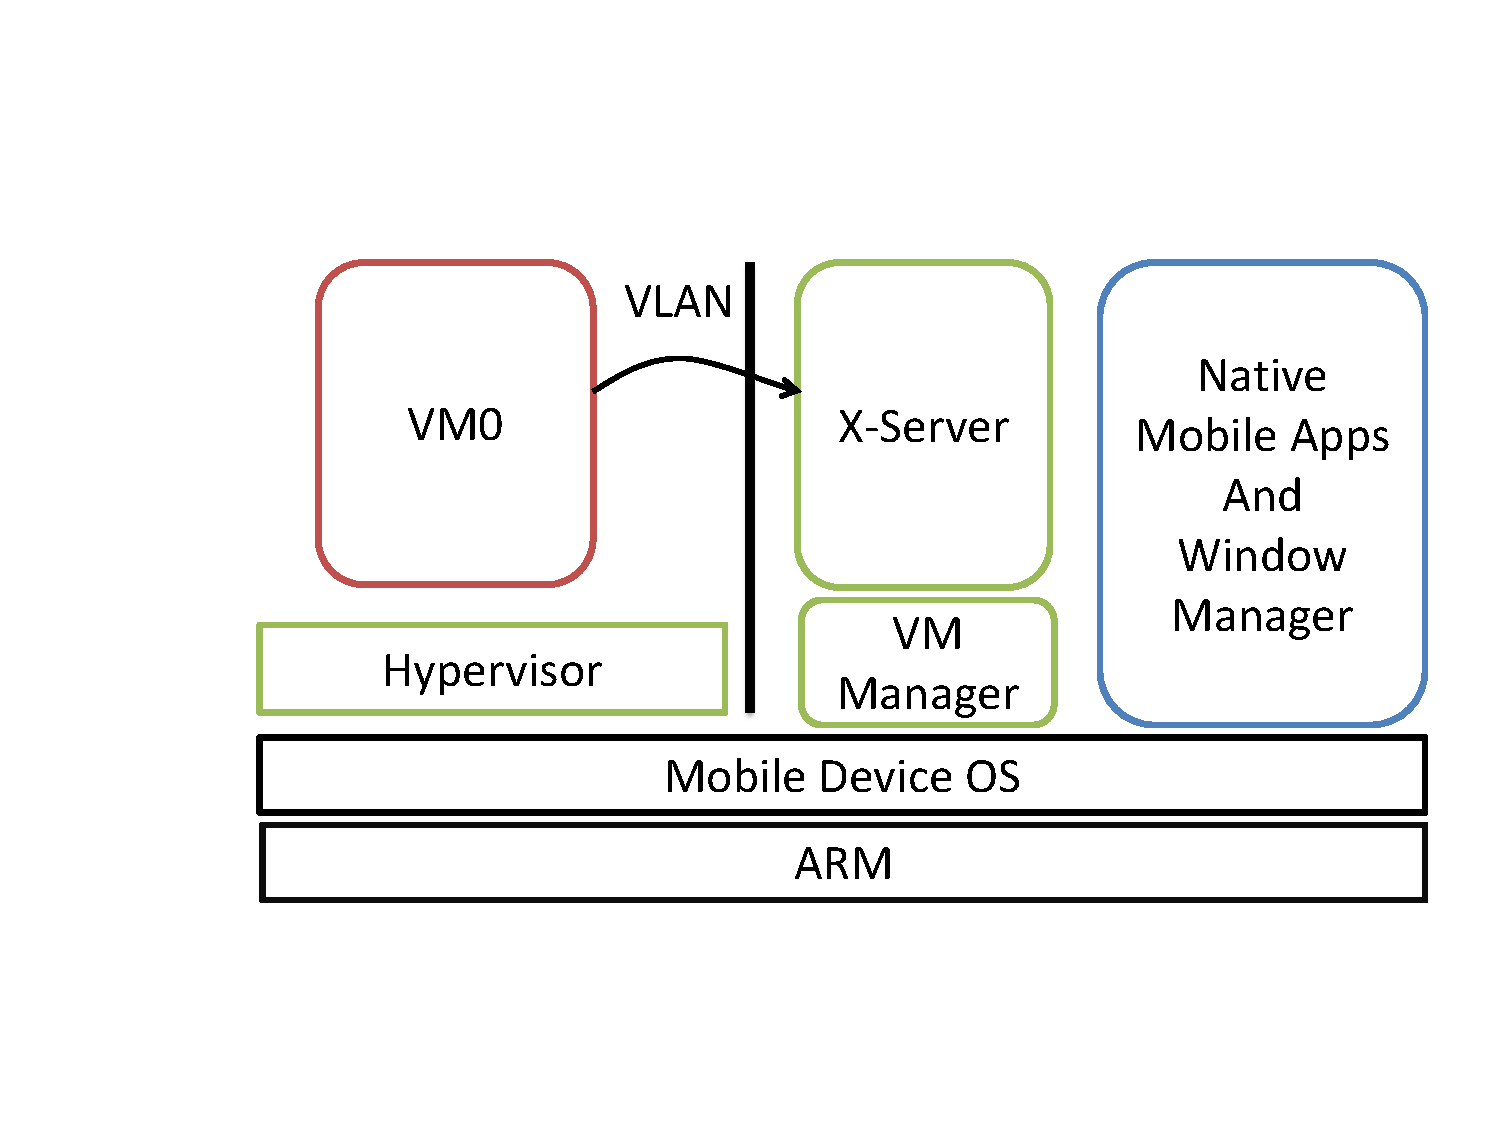
\includegraphics[width=1.0\columnwidth]{arch}
\caption{Architecture diagram}
\label{fig:arch}
\end{figure}

\subsection{Proposed Architecture}
\label{sec:proposedarch}
%Here describe what we propose to do, perhaps?
%Our timeline/evaluation are kinda worthless without it.
Our proposed architecture has two main components: the virtualization framework, and the integration front-end.  The virtualization framework contains the hypervisor (QEMU or KVM based) as well as each of the spawned VM's (see Figure \ref{fig:arch}).  Each VM will contain a thin OS for running the third-party application.  We can choose either to run an x86-based Operating Systems in the VM or an ARM based Operating System. The former will enable a more diverse set of target applications to be run, while the latter would have lesser overhead due to virtualization. We plan to evaluate both of these options. Each of the VM's will headless themselves, but will render their applications by connecting to the native X server. \\

The other component is the integration front-end.  This contains a light X server that has been integrated into the host OS, and also contains the VM manager.  The VM manager will either run inside the X-server as a native application (ARM-based), or as a separate application within the host OS.  The VM manager will be the user interface that controls launching, switching, suspending, resuming, migrating the VM's and ensuring the X-server is running properly. Note that most of this actual logic and functionality will be implemented by the hypervisor in the virtualization framework.\\

The shared X-server allows us to share the rendering of the applications, which is an improvement over running an X-server in each of the VM. We plan to use different X-sessions per VM to reduce sharing between them.
Additionally the X-server will be running native code, which will allow for it to be less cpu-intensive than it might otherwise. \\

Additionally we aim to have the virtualization framework be device independent, which is important because we anticipate this to be the more complex component.  The integration front-end will have to be ported for each new device we support, but we will strive to make implementation simple. Our first implementation will focus on one particular device and OS as well as the supportfor live migration of applications from desktops. \\

In summary, we propose to leverage existing hypervisors to build a secure, usable and portable framework for mobile device virtualization. Our contributions will be focused on providing the ability for live migration of applications with deep integration to the mobile device. Our security model proposes an effective method of isolatng applications and find that our design ideas are similar to other recent efforts \cite{grier2008secure} in isolating untrusted code.
